\chapter{The Nature And Eradication Of Fear}

This chapter follows J. Krishnamurti's San Diego dialogue with Dr. Alan W. Anderson on the nature and eradication of fear. Source credit belongs to J. Krishnamurti and the Krishnamurti Foundation Trust material; this course chapter is curated by LazyingArt LLC through Video2Book. The displayed formulas and diagrams below are not blackboard mathematics. They are compact schematic aids for preserving the order of the inquiry: fear is first encountered in its many forms, then questioned at its root, and finally seen in relation to thought, intelligence, knowledge, and freedom.

\section{The Whole Movement Of Fear}

The dialogue resumes exactly where the previous conversation had left a question open. Anderson recalls that they had come to the point where fear arose, and Krishnamurti agrees that they should explore it together. He does not begin by defining fear. He begins by widening the field. Fear may be fear of death, fear of loneliness, fear of not being loved, fear of not becoming successful, fear of losing physical security. The opening movement is important: fear is not treated as a private symptom, but as a common human fact.

At the same time, Krishnamurti places fear beside pleasure. The two are called two sides of the same coin. Pleasure will be taken up later, but it is already named because fear is not being examined as an isolated emotion. It belongs to a larger movement of pursuit, memory, desire, and avoidance. We can mark that pairing schematically as

\begin{equation}
\text{fear} \leftrightarrow \text{pleasure}.
\end{equation}

This is not a scientific equation. It is a reminder of the lecture's architecture: fear is the object of this conversation, but pleasure is waiting on the other side of it.

Krishnamurti then proposes a method. We should begin with outward, physical fear and move inward. That sequence protects the inquiry from becoming too abstract too soon. Before asking what fear is at its root, we must see the field in which it operates. Let \(F\) denote, only as notation for these notes, the whole movement of fear. Then the first partition is

\begin{equation}
F = F_{\mathrm{physical}} \cup F_{\mathrm{psychological}}.
\end{equation}

Here \(F_{\mathrm{physical}}\) includes fears bound up with food, clothing, shelter, work, pain, survival, and death. \(F_{\mathrm{psychological}}\) includes fear of loneliness, dependency, rejection, image, public opinion, achievement, not being, and identification. The notation is useful only if we remember Krishnamurti's later correction: these two regions are not sealed compartments. Physical and psychological fear are interrelated.

\section{Physical Security And The Disorder Of Division}

The first serious example is security. The brain, Krishnamurti says, needs security as a child needs security. Without security, action becomes distorted, unhealthy, neurotic, lopsided. Food, clothing, and shelter are therefore not secondary matters. They are necessary conditions for sane human functioning.

But the inquiry immediately becomes paradoxical. We require security, yet we organize life in ways that destroy it. National division, sovereign governments, armies, competition, and economic dependence all enter the discussion. A job gives a sense of security, but that job depends on production, business, consumerism, competition with other countries, and the whole commercial structure. The mind wants security and at the same time participates in structures that deny security.

The contradiction can be kept before us in a compressed form:

\begin{align}
\text{brain} &\longrightarrow \text{requires security}, \\
\text{division}+\text{competition}+\text{war} &\longrightarrow \text{destruction of security}.
\end{align}

This is the first major turn. Krishnamurti is not adding political commentary to a psychological lecture. He is showing that disorder is not elsewhere. The same mind that seeks security also separates itself as nation, class, belief, occupation, and image. It then wonders why security cannot be found.

The examples remain concrete: losing a job, seeing poverty, living with hunger, making plans more important than starvation. These examples are not ornaments. They are the way the lecture moves from the outward fact of security toward the inward movement of fear.

\section{Outer Fear Becomes Inner Fear}

The next transition is physical pain. One has had pain, perhaps last week, and the mind is afraid it may happen again. Anderson notices that what is remembered is not only a bodily event but the emotion that attended it. Krishnamurti accepts the point and continues. Fear has begun to show its relation to memory and time.

\paragraph{Worked example: remembered pain.}
The sequence can be written as a small derivation, provided we keep it schematic:

\begin{enumerate}
\item A physical pain occurs.
\item Memory carries the emotional trace of that pain.
\item Thought projects recurrence: it may happen again.
\item The projected recurrence is experienced now as fear.
\end{enumerate}

Thus,

\begin{equation}
\text{pain}_{\mathrm{past}}
+\text{memory}
+\text{projection into tomorrow}
\longrightarrow
\text{fear now}.
\end{equation}

The point is not that pain equals fear. Pain may be a fact. Fear arises when memory and projection carry that fact forward as possible repetition.

From pain, the dialogue moves to public opinion, reputation, and image. What will my neighbour say? What will society think? If a person depends on the neighbour for respectability, position, or work, then the neighbour's opinion becomes a source of fear. Krishnamurti's examples are deliberately ordinary. A person may salute what he inwardly does not believe because his social and economic position depends upon it. The image governs conduct.

The outward and inward are now visibly entangled. A job is outward; dependence on respectability is inward. Poverty is outward; hopelessness enters the mind. Public opinion is outward; the image of oneself is inward. The lecture has not yet named thought as the root, but the path is being prepared.

\section{Dependency, Loneliness, And Identification}

The inward fears are more complicated. Dependency is central. I depend on my wife, my husband, my guru, my priest, my belief, my country, my image. If that person turns away, if that belief fails, if that image is threatened, I am frightened. Jealousy, anger, violence, and anxiety may follow because what I called relationship was partly dependence.

Then comes loneliness. To avoid loneliness one may attach oneself to another person, to a belief, to a saviour, to a guru, to an ideology. Anderson describes this as filling the hole with a new image. Krishnamurti's response is severe: the image does not end fear. It is another form of the same disorder.

A useful schematic is

\begin{equation}
\text{loneliness}
\longrightarrow
\text{attachment}
\longrightarrow
\text{dependence}
\longrightarrow
\text{fear of loss}.
\end{equation}

The same movement appears in achievement. There is fear of not arriving, not succeeding, not becoming enlightened, not expanding consciousness, not being somebody. The fear of not being translates itself into identification: with country, with God, with an invented image of oneself. Krishnamurti reverses a familiar religious formula: God has not made man in his image; man has made God in his image.

At this point the lecture has accumulated many fears: logical fears, irrational fears, neurotic fears, survival fears, hidden fears. The list is intentionally heavy. It creates the next question.

\subsection{Question \& Answer}

\paragraph{Question.}
Can fear be dealt with one item at a time? Can we take loneliness, public opinion, physical pain, death, dependency, and each separate fear in turn?

\paragraph{Answer.}
Krishnamurti's answer is no. To deal with fear one branch after another is to spend a lifetime pruning leaves while the root remains untouched. Anderson calls this the round of fragmentation. Krishnamurti adds that analysis itself becomes paralysis: I analyse fear, then fear that the analysis may be incomplete, then seek further analysis, and the movement continues.

The failed rule is

\begin{equation}
\{f_1,f_2,\ldots,f_n\}
\longrightarrow
\text{fragmented analysis}
\longrightarrow
\text{paralysis}.
\end{equation}

The alternative is not faster analysis. It is a different order of question:

\begin{equation}
\text{many fears}
\longrightarrow
\text{whole movement of fear}
\longrightarrow
\text{root inquiry}.
\end{equation}

We stop asking how to manage each branch and begin to ask what fear is.

\begin{figure}
\centering
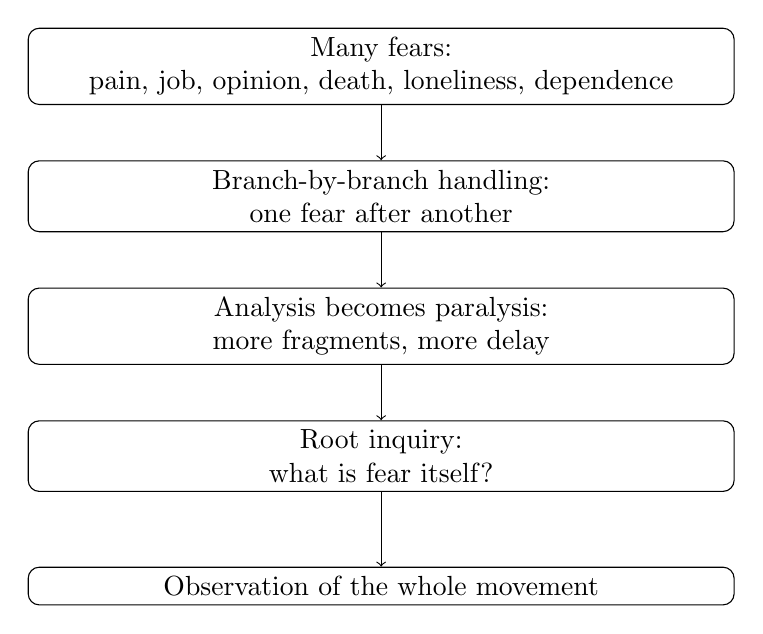
\begin{tikzpicture}
\node[draw, rounded corners, align=center, text width=0.72\linewidth] (many) at (0,0) {Many fears:\\ pain, job, opinion, death, loneliness, dependence};
\node[draw, rounded corners, align=center, text width=0.72\linewidth] (branch) at (0,-1.65) {Branch-by-branch handling:\\ one fear after another};
\node[draw, rounded corners, align=center, text width=0.72\linewidth] (paralysis) at (0,-3.30) {Analysis becomes paralysis:\\ more fragments, more delay};
\node[draw, rounded corners, align=center, text width=0.72\linewidth] (root) at (0,-4.95) {Root inquiry:\\ what is fear itself?};
\node[draw, rounded corners, align=center, text width=0.72\linewidth] (observe) at (0,-6.60) {Observation of the whole movement};
\draw[->] (many) -- (branch);
\draw[->] (branch) -- (paralysis);
\draw[->] (paralysis) -- (root);
\draw[->] (root) -- (observe);
\end{tikzpicture}

\paragraph{Schematic reconstruction.}
From fragmented fears to root inquiry.
\end{figure}

\section{What Is Fear When Escape Ends?}

Now Krishnamurti refuses description. Fear is not to be found by naming its objects or repeating explanations. What is fear behind the words, behind the description, behind the ways out and the ways in? Anderson notices that his own academic response is inadequate. To say, ``if I have followed you,'' and then offer a formulation is already to stand away from the fact. Fear has to be found as directly as hunger is found.

The rhythm slows here. Krishnamurti removes the ordinary exits one by one: no escape, no rationalization, no analysis, no backing off, no explanatory refuge. The negation is not emptiness or passivity. It clears the field so that the fact can be met.

Then he introduces hidden fear. Can the conscious mind invite hidden fears to the surface? His answer is cautious. Conscious thought can deal with what it knows, but it cannot observe the thing it does not know. Dreams are mentioned and set aside as a continuation of daily movement in another form. The sharper question is how hidden fears -- racial fears, inherited fears, fears imposed by society, family, and neighbour -- can be exposed naturally, so that the mind sees them completely.

Anderson then makes the dialogue itself an example. In a university setting, one may sit listening while secretly preparing a response, protecting reputation, wondering whether one appears intelligent. Fear prevents listening. The professor's image is at stake. Thus the question of hidden fear is no longer remote; it is present in the very act of conversation.

\subsection{Question \& Answer}

\paragraph{Question.}
If analysis cannot expose hidden fear, and escape has been seen as futile, what action remains?

\paragraph{Answer.}
Krishnamurti's answer begins with negation. Escape, analysis, rationalization, identification, resistance, and refuge in authority are seen as futile. When those movements end, energy is no longer dissipated. This energy is not physical energy and not a mystical possession. It is the gathered intensity of attention when the usual leaks have stopped.

We may write the relation as

\begin{equation}
\neg(\text{escape}+\text{analysis}+\text{identification}+\text{resistance})
\longrightarrow
\text{undissipated energy}.
\end{equation}

But then he blocks another false turn. When faced with fear, we ask, ``What can I do?'' His answer is: I cannot do anything. The ``I'' that wants to act is itself implicated in the production of fear. Public opinion, image, dependency, identification, and the demand to become something are not merely external objects. They are part of the movement of self.

So the question changes again. Not: what shall I do to fear? But: what has brought fear about?

\section{Thought, Recognition, And The Observer}

The inquiry now becomes exact. What has created fear? My neighbour? My country? My culture? Myself? Krishnamurti does not accept a merely verbal answer. The answer must be seen.

The decisive question is whether the mind can observe fear, not one piece of fear and not a succession of fears, but the whole movement of fear. Can there be observation without the thought that has created the observer?

The compact identity for this passage is

\begin{equation}
\text{observer} = \text{thought}.
\end{equation}

This should be read carefully. It is not a general metaphysical formula. It preserves the lecture's claim that the observer who says, ``I am afraid,'' is not separate from the movement of thought that recognizes, names, remembers, and projects fear.

The process can be represented as follows:

\begin{align}
\text{previous experience} &\longrightarrow \text{recognition}, \\
\text{recognition} &\longrightarrow \text{naming: ``fear''}, \\
\text{naming}+\text{memory} &\longrightarrow \text{projection}, \\
\text{projection} &\longrightarrow \text{fear sustained}.
\end{align}

Krishnamurti keeps the point concrete. I am afraid of what my neighbour says because I want to be respectable. Thought has divided the world into nations and thereby destroyed physical security. I am lonely, and thought seeks neurotic escape through attachment. I had pain yesterday, and thought projects it into tomorrow. In each case, thought nourishes fear.

A subtle distinction follows. Fear is new each time, but it is made old when recognized. Recognition belongs to the past, to knowledge, to association. When the mind names the present fact by carrying over what has been, it gives continuity to fear.

The ending is stated without ornament:

\begin{equation}
\text{observation without the observer}
\longrightarrow
\text{fear is not}.
\end{equation}

This must not be turned into a technique. It is not a method to practise in order to obtain a result. In the lecture, it comes only after seeing the whole movement of fear and the whole movement of thought.

\begin{figure}
\centering
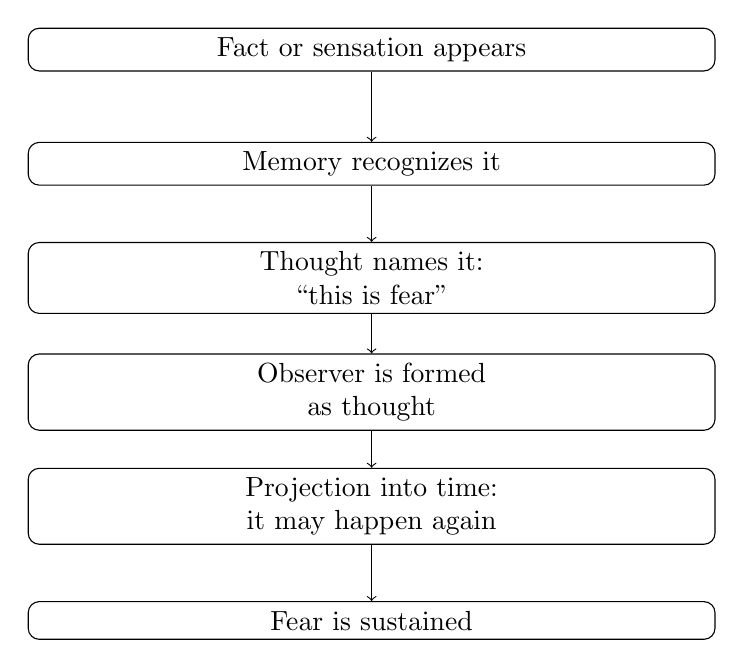
\begin{tikzpicture}
\node[draw, rounded corners, align=center, text width=0.70\linewidth] (fact) at (0,0) {Fact or sensation appears};
\node[draw, rounded corners, align=center, text width=0.70\linewidth] (memory) at (0,-1.45) {Memory recognizes it};
\node[draw, rounded corners, align=center, text width=0.70\linewidth] (name) at (0,-2.90) {Thought names it:\\ ``this is fear''};
\node[draw, rounded corners, align=center, text width=0.70\linewidth] (observer) at (0,-4.35) {Observer is formed\\ as thought};
\node[draw, rounded corners, align=center, text width=0.70\linewidth] (projection) at (0,-5.80) {Projection into time:\\ it may happen again};
\node[draw, rounded corners, align=center, text width=0.70\linewidth] (sustain) at (0,-7.25) {Fear is sustained};
\draw[->] (fact) -- (memory);
\draw[->] (memory) -- (name);
\draw[->] (name) -- (observer);
\draw[->] (observer) -- (projection);
\draw[->] (projection) -- (sustain);
\end{tikzpicture}

\paragraph{Schematic reconstruction.}
Recognition, naming, and projection as the sustaining movement of psychological fear.
\end{figure}

\section{Intelligence, Knowledge, And Freedom}

Krishnamurti then protects the inquiry from a misunderstanding. If a bus rushes toward us, or if we see a dangerous animal, we move. That movement is not psychological fear in the sense being examined. It is intelligent self-protection. Intelligence acts directly in the face of danger.

\begin{table}
\centering
\begin{tabular}{p{0.43\linewidth}p{0.43\linewidth}}
\textbf{Self-protective intelligence} & \textbf{Psychological fear} \\
Immediate response to danger & Fear of public opinion \\
Moving away from a rushing bus & Fear of recurring pain through memory \\
Action without inner narrative & Loneliness sustained by image and attachment \\
Intelligence operating in fact & Thought projecting past into future \\
\end{tabular}

\paragraph{Schematic distinction.}
The lecture separates practical self-protection from psychological fear.
\end{table}

This distinction is essential. The inquiry is not asking human beings to ignore danger. It is asking whether the other movement -- the movement of thought, image, recognition, and projection -- can end.

Krishnamurti then asks whether thought can understand itself, know its place, and not project itself. Control is rejected. If thought controls thought, the controller is another fragment of thought. The game has no end.

\paragraph{Worked example: knowledge in its place.}
The final passage turns on the place of knowledge.

\begin{enumerate}
\item Practical knowledge is necessary: language, driving, science, mathematics, ordinary skill.
\item Psychological knowledge is accumulated conditioning: image, tradition, respectability, experience used as authority.
\item When psychological knowledge tries to understand fear, it turns the living fact into something old.
\item To understand what is, accumulated psychological knowledge has no transforming power.
\item Therefore freedom from fear is not produced by knowledge.
\end{enumerate}

The notation is

\begin{align}
K_{\mathrm{practical}} &\neq K_{\mathrm{psychological}}, \\
K_{\mathrm{psychological}} &\not\Rightarrow \text{freedom from fear}.
\end{align}

This is the lecture's final clarification of thought's proper place. Knowledge is necessary where knowledge belongs. Speaking a language, driving, science, mathematics, and ordinary technical action require it. But the accumulated knowledge of psychological experience, tradition, respectability, and fear has no value in the transformation of fear. In this field, knowledge becomes ignorance.

Krishnamurti closes by saying that freedom is not born of knowledge. Freedom is not another object to pursue, and it is not something placed where fear used to be. It comes when the burden is not.

\begin{equation}
\text{freedom} \notin K,
\qquad
\text{freedom appears when burdens are absent}.
\end{equation}

The statement has to remain austere. Nothing compensatory is put in the place of fear. No new image is offered. When thought, as observer, no longer sustains the movement, fear is not.

\section{Summary}

The dialogue moves from the many forms of fear to the whole movement of fear. It begins with physical security and shows how human division destroys the very security the brain needs. It then moves through pain, public opinion, poverty, dependency, loneliness, achievement, and identification until the list itself becomes impossible to handle one item at a time.

That impossibility produces the root question. Analysis of fragments is paralysis. Escape, rationalization, identification, and resistance dissipate energy. When those movements are seen as futile, there is energy to ask what has brought fear about.

The answer is not a definition but a seeing. Thought, through memory, recognition, naming, projection, and the observer, sustains psychological fear. Intelligent self-protection is different; it acts directly when there is danger. Practical knowledge has its place, but accumulated psychological knowledge cannot transform fear. Freedom is not born of knowledge. It is present when the burden carried by thought is no longer there.